\begin{figure*}
  \centering
  \begin{subfigure}{0.14\linewidth}
    \centering
    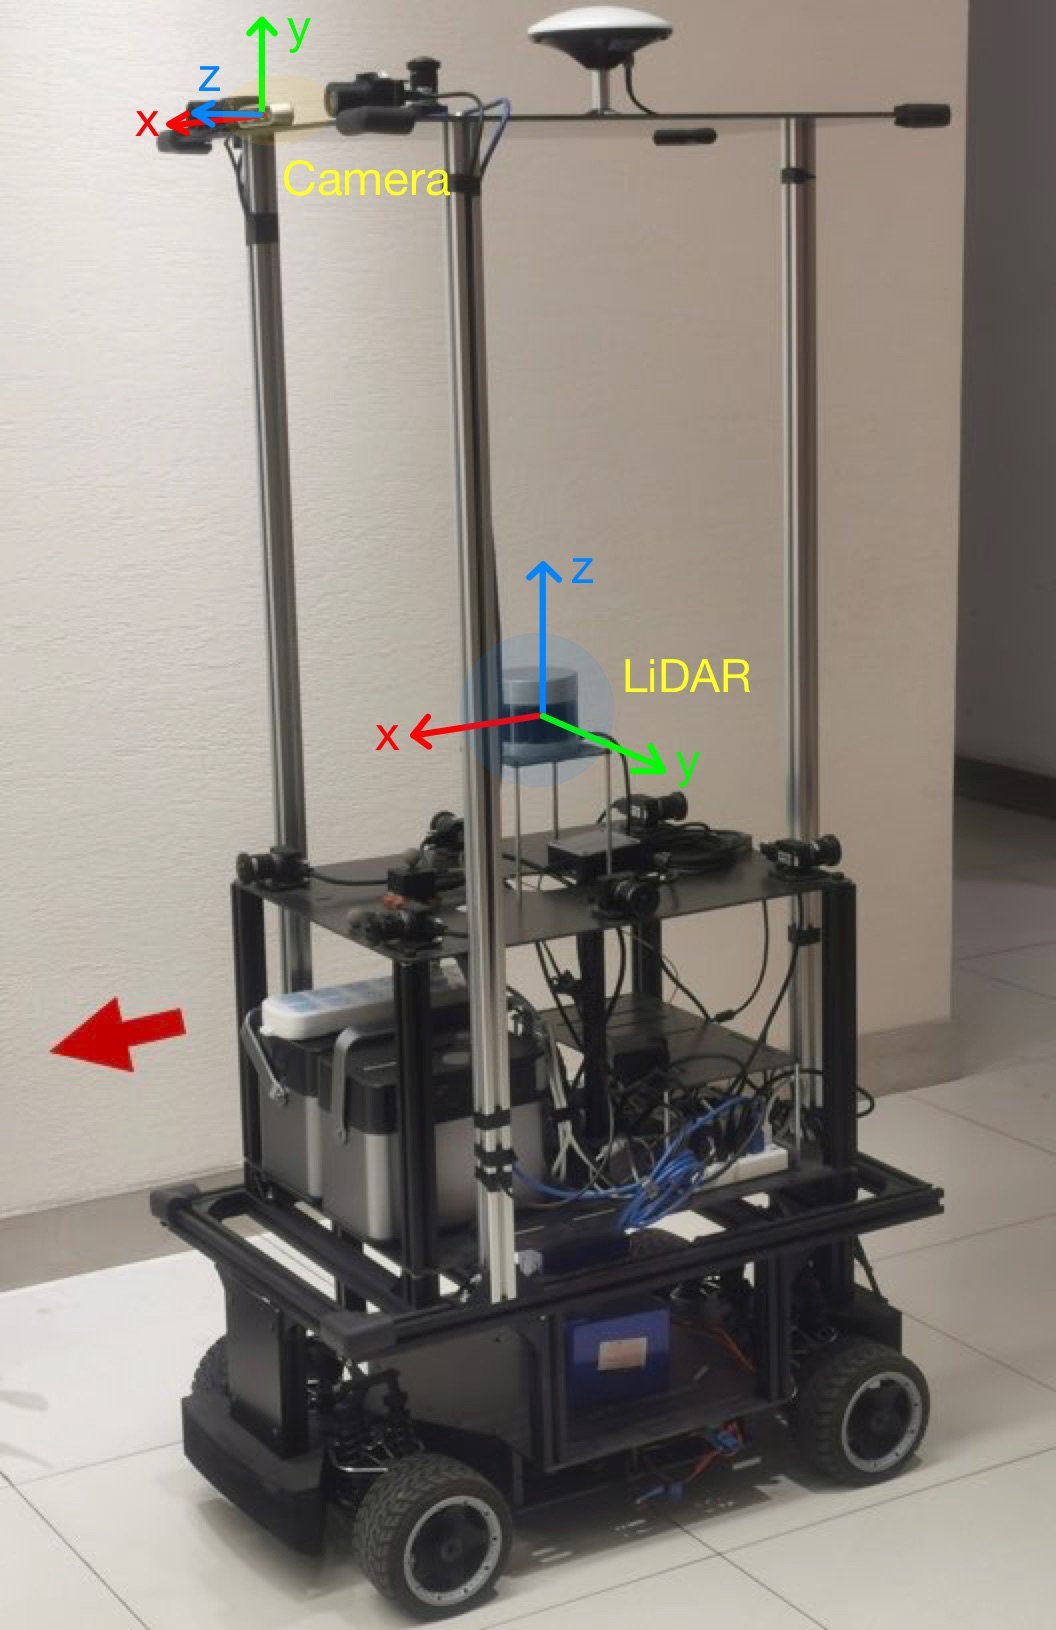
\includegraphics[width=\linewidth]{images/ground_robot.jpg}
    \caption{Ground robot}
    \label{fig:ground_robot}
  \end{subfigure}
  \hfill
  \begin{subfigure}{0.28\linewidth}
    \centering
    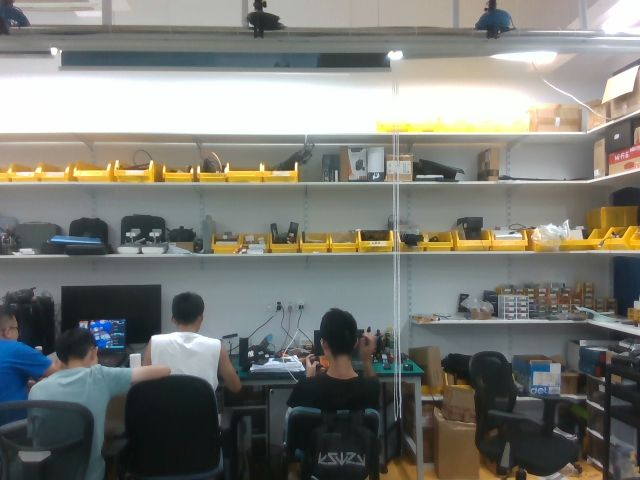
\includegraphics[width=\linewidth]{images/room.png}
    \caption{Indoor scene: room}
    \label{fig:room}
  \end{subfigure}
  \begin{subfigure}{0.28\linewidth}
    \centering
    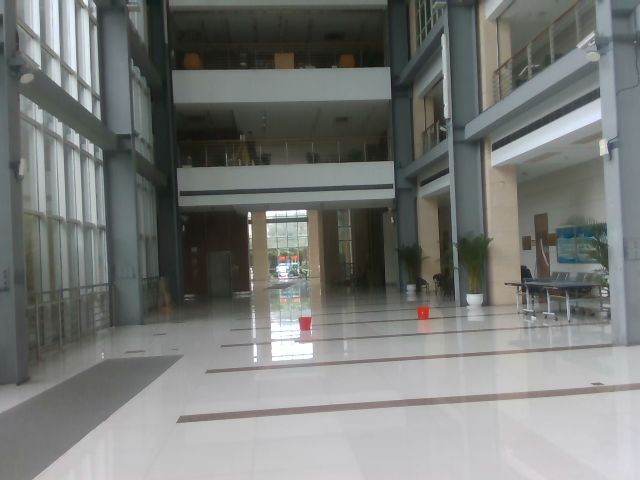
\includegraphics[width=\linewidth]{images/hall.png}
    \caption{Indoor scene: hall}
    \label{fig:hall}
  \end{subfigure}
  \begin{subfigure}{0.28\linewidth}
    \centering
    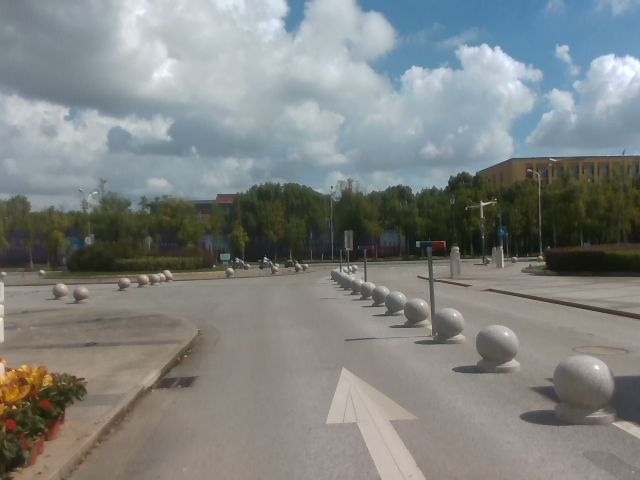
\includegraphics[width=\linewidth]{images/outdoor.png}
    \caption{Outdoor scene: gate}
    \label{fig:outdoor}
  \end{subfigure}

  \caption{An overview of the mobile agent and scenes in the M2DGR dataset~\cite{yin2021m2dgr} to accomplish the dual-system SLAM.}
  \label{fig:dataset}
  \vskip -3ex
\end{figure*}

\begin{table}
\centering
\begin{tabular}{cccc}
\toprule
Sequence & Structure PLP~\cite{shu2022structure} & MULLS~\cite{pan2021mulls} & Ours\\
\hline
room\_01 & 0.1233 & 0.1446 & \textbf{0.0848} \\
room\_02 & 0.2063 & 0.1197 & \textbf{0.0996} \\
room\_03 & 0.1143 & 0.1620 & \textbf{0.1075} \\
\hline
hall\_02 & $\times$ & 0.3612 &  \textbf{0.3517} \\
hall\_03 & $\times$ & 0.6820 &  \textbf{0.5975} \\
hall\_04 & $\times$ & 0.9049 &  \textbf{0.8886} \\
\hline
gate\_01 & $\times$ & 0.7322 & \textbf{0.6395} \\
gate\_02 & $\times$ & 0.3916 & \textbf{0.2954} \\
gate\_03 & $\times$ & 0.4165 & \textbf{0.3211} \\
\hline
\end{tabular}
\caption{Comparison experiments with the single-modality baselines on the M2DGR~\cite{yin2021m2dgr}, where results are presented in terms of the aligned mean translation error (m). If the method fails to initialize or track frames less than half of the total frames, we mark it ``$\times$''.}
\label{tab:table_baseline}
\vskip -3ex
\end{table}

We use the M2DGR dataset~\cite{yin2021m2dgr} to evaluate the leveraged approaches. All experiments were performed on an i5-8260U laptop with $16$ GB memory. Our method is compared with diverse baselines, \ie,  Structure PLP-SLAM~\cite{shu2022structure}, MULLS~\cite{pan2021mulls}, and other multi-modal SLAM algorithms ORB-SLAM3~\cite{campos2021orb} and LVI-SAM~\cite{shan2021lvi}. 

\subsection{Introduction regarding the M2DGR dataset}
This dataset includes indoor and outdoor sequences captured using a LiDAR sensor and a monocular camera mounted on a ground robot, as shown in Figure~\ref{fig:dataset}. The indoor applications of robots are often found in offices, where dynamic objects (people) interfere with the robot's work. Therefore, it is necessary to update the map by SLAM. Mobile robots also guide visitors to their defined destinations within the hall.
SLAM provides directions and can find important landmarks to assist the robot. Besides indoor scenes, mobile robots are widely utilized for various domains, \textit{e.g.}, logistics operations and package transportation, where SLAM helps in navigation.
%
And their night-time work not only optimizes human resources but also guarantees efficient and timely deliveries.

To explore the diversity of mobile robot applications, we select three scenarios where mobile robots are commonly employed: the texture-rich office, the spacious orderly hall, and outdoor scenes with varying lighting conditions. 

\subsection{Comparison with the single-modal SLAMs} 

In the scenario room, each frame has numerous feature points and lines. The trajectories shown in Figure~\ref{fig:room_vs_base} demonstrate that our system successfully achieves pose estimation. Compared with Structure PLP and MULLS- in Table~\ref{tab:table_baseline}, our method delivers superior accuracy.

The hall scene is an ideal environment for geometry-based visual SLAM due to its regular structure. However, the motion blur in this scene poses a challenge to visual SLAM which has a problem with tracking enough feature points. A similar problem occurs in outdoor scenes, where distant landmarks occupy only small portions of the captured images due to the wider field of view and longer range. In addition, certain sequences in outdoor scenes are collected at night, further exacerbating the problem. In such situations, the visual SLAM system can not detect adequate feature points, leading to tracking failures. Consequently, both the Structure PLP and our visual subsystem face limitations in estimating the entire odometry in these scenarios.

LiDAR has long-range sensing capability and stability in various lighting conditions. It always provides accurate and reliable trajectory estimation. The performance of our LiDAR subsystem is shown in Table~\ref{tab:table_baseline} and in Figures~\ref{fig:hall_vs_base}, \ref{fig:gate_vs_base}. The fusion framework enhances its linear direction, increasing the accuracy of the odometry.

\begin{figure*}
  \centering
  \begin{subfigure}{0.24\linewidth}
    \centering
    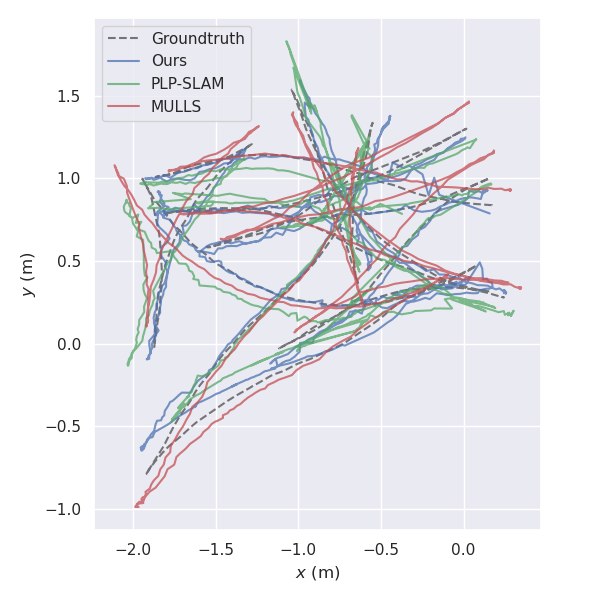
\includegraphics[width=\linewidth]{images/room_01_trajectories.png}
    \caption{Sequence: room\_01}
    \label{fig:room_vs_base}
  \end{subfigure}
  \begin{subfigure}{0.24\linewidth}
    \centering
    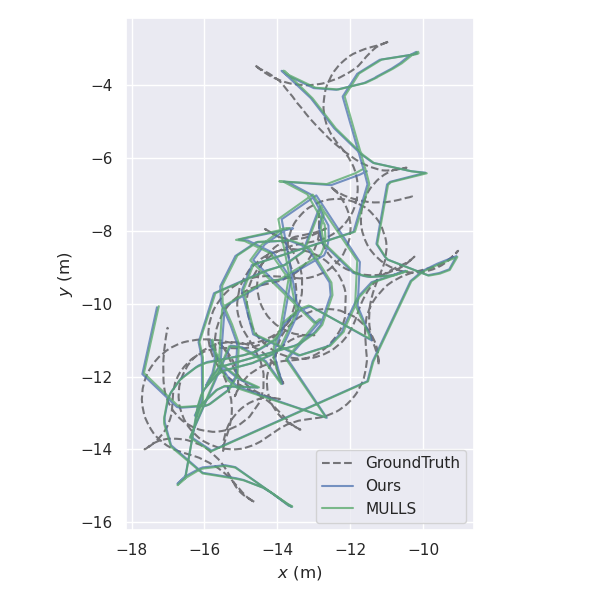
\includegraphics[width=\linewidth]{images/hall_03_trajectories.png}
    \caption{Sequence: hall\_03}
    \label{fig:hall_vs_base}
  \end{subfigure}
  \begin{subfigure}{0.24\linewidth}
    \centering
    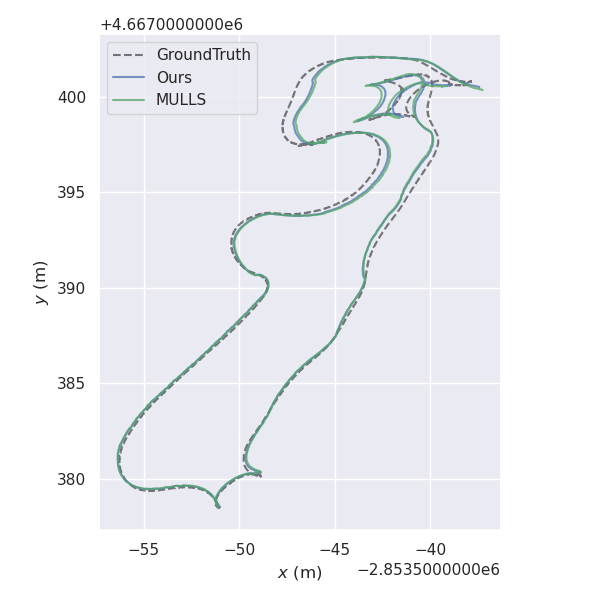
\includegraphics[width=\linewidth]{images/gate_01_trajectories.png}
    \caption{Sequence: gate\_01}
    \label{fig:gate_vs_base}
  \end{subfigure}
  \begin{subfigure}{0.24\linewidth}
    \centering
    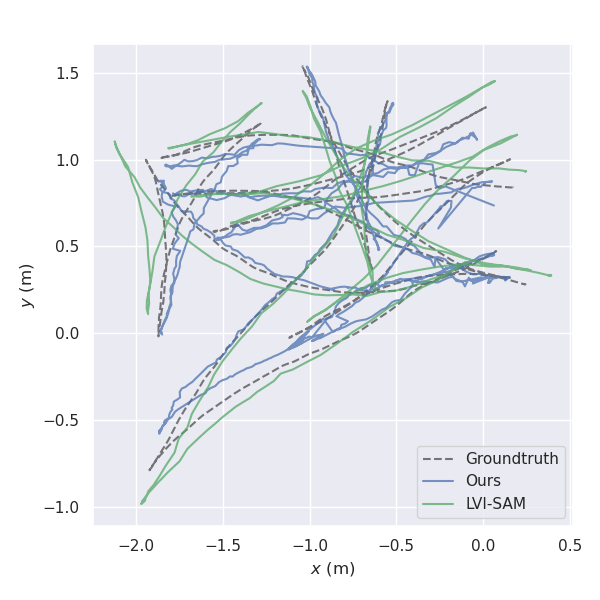
\includegraphics[width=\linewidth]{images/vs_LVI.png}
    \caption{Sequence: room\_01}
    \label{fig:room_vs_sota}
  \end{subfigure}
  \caption{The comparison regarding the trajectories 
 of the indoor/outdoor scenes. (a), (b), and (c) compare our method with Structure PLP~\cite{shu2022structure} and MULLS~\cite{pan2021mulls} while (d) compares our method with the other multi-modal SLAM, \ie,  LVI-SAM~\cite{shan2021lvi}.}
  \label{fig:dataset_sequences}
  \vskip -3ex
\end{figure*}

\begin{table}
\centering
\begin{tabular}{cccc}
\toprule
Sequence& LVI-SAM \cite{shan2021lvi} & ORB-SLAM3 \cite{campos2021orb} & Ours \\
\hline
room\_01 & 0.1498 & $\times$ &  \textbf{0.0848} \\
room\_02 & 0.1176 & $\times$ & \textbf{0.0996} \\
room\_03 & 0.1588 & $\times$ & \textbf{0.1075} \\
\hline
hall\_04 & \textbf{0.8037} & $\times$  &  0.8886 \\
\hline
gate\_02 & 0.3080  & $\times$  & \textbf{0.2954} \\
gate\_03 & \textbf{0.1198} &  $\times$ & 0.3211 \\
\hline
\end{tabular}
\caption{Comparison experiments with the multi-modal SLAMs LVI-SAM~\cite{shan2021lvi} and ORB-SLAM~\cite{campos2021orb} on the M2DGR dataset~\cite{yin2021m2dgr}, where results are presented in terms of the aligned mean translation error (m).}
\label{tab:table_other_method}
\vspace{-3mm}
\end{table}

\subsection{Comparison with the multi-modal SLAMs} 

Due to the limited availability of open-source LiDAR-visual SLAM algorithms in recent years, we choose two well-established multi-modal algorithms for comparison: the visual-inertial-LiDAR SLAM, LVI-SAM~\cite{shan2021lvi} and the visual-inertial SLAM, ORB-SLAM3~\cite{campos2021orb}.
Comparing the outdoor sequences in Table~\ref{tab:table_other_method}, LVI-SAM, which integrates data from the IMU, camera, and LiDAR sensors, harvests more accurate visual-enhanced LiDAR odometry. The visual-inertial algorithm ORB-SLAM3 suffers from significant drift and then tracking failures in all scenarios. Despite utilizing only two sensors, our method achieves higher accuracy and robustness in both indoor and outdoor scenes, as illustrated in Figure~\ref{fig:room_vs_sota}.